\documentclass[11pt]{article}
%%%%%%%%%%%% PREAMBULO %%%%%%%%%%%%%%%%%%
\usepackage[T1]{fontenc}%indica que usamos la ñ
\usepackage[utf8]{inputenc}%indica el tipo de codificación ISO-8859-1 (latin)ó utf8
\usepackage[spanish]{babel}%indica que escribiremos en español
\title{plantilla para reportes mecatrónica-mecánica UTA}
\usepackage{amsmath}
\usepackage{amssymb,amsfonts,latexsym}
\usepackage{graphicx}
\usepackage{epstopdf}%para convertir figuras a formato pdf
\usepackage{color}
\usepackage{url}  \urlstyle{same}%para conectar url strings en bibliografías
\usepackage{subfigure}%para colocar varias figuras
\usepackage{multicol}
\usepackage{changepage}
\usepackage{float}%para colocar las tablas como H
\usepackage{array}%dar formato a las tablas
\usepackage{longtable}%dar formato a las tablas
\usepackage{bm}
\usepackage{capt-of}
\usepackage{sidecap}
\sidecaptionvpos{figure}{c}
\usepackage{caption}
\usepackage{commath}
\usepackage{cancel}
\usepackage{lipsum}
%%%%%%%%%%% CONFIGURACION DEL DOCUMENTO %%%%%%%%%%%%%
\usepackage{anysize}%para personalizar el ancho de los margenes
\marginsize{2cm}{2cm}{2cm}{2cm}%izquierda, derecha, arriba, abajo
\usepackage{anyfontsize}

% Para que las referencias sean hipervínculos a las figuras o ecuaciones y
% aparezcan en color
\usepackage[colorlinks=true,plainpages=true,citecolor=blue,linkcolor=blue]{hyperref}
%\usepackage{hyperref} 
% Para agregar encabezado y pie de página
\usepackage{fancyhdr} 
\pagestyle{fancy}
\fancyhf{}
\fancyhead[L]{\footnotesize FICH} %encabezado izquierda
\fancyhead[R]{\footnotesize Centis Mateo}   % dereecha
\fancyfoot[R]{\footnotesize Entregable 1}  % Pie derecha
\fancyfoot[C]{\thepage}  % centro
\fancyfoot[L]{\footnotesize Ingeniería en informática}  %izquierda
\renewcommand{\footrulewidth}{0.4pt}
\usepackage{listings} % Para usar código fuente

% configuración para el lenguaje que queramos utilizar
\definecolor{mygreen}{rgb}{0,0.6,0}
\definecolor{mygray}{rgb}{0.5,0.5,0.5}
\definecolor{mymauve}{rgb}{0.58,0,0.82}
\definecolor{myorange}{rgb}{0.855,0.576,0.027}
\definecolor{backcolour}{rgb}{0.95,0.95,0.92}
\lstset{
language=Octave,
frame=single,   
morecomment = [l][\itshape\color{mygreen}]{\%},
keywordstyle=\color{blue},
commentstyle=\color{mygreen},	
breakatwhitespace=false,         
breaklines=true,  
%numbers=left,
%numbersep=5pt,
basicstyle=\linespread{0.9}\ttfamily\small,
%numberstyle=\tiny\color{mygray}, 
showstringspaces=false, 
showtabs=false,                  
tabsize=2,
stringstyle=\color{myorange},
title=\lstname,
literate=
{+}{{{\color{red}+}}}1
{-}{{{\color{red}-}}}1
{*}{{{\color{red}*}}}1
{,}{{{\color{red},}}}1
{=}{{{\color{red}=}}}1
{)}{{{\color{red})}}}1
{(}{{{\color{red}(}}}1 
{;}{{{\color{red};}}}1
{:}{{{\color{red}:}}}1
{[}{{{\color{red}[}}}1
{]}{{{\color{red}]}}}1
{>}{{{\color{red}>}}}1
}
\title{Plantilla para informes ing. mecanica-mecatronica}

%%%%%%%%%%% COMIENZO DEL DOCUMENTO %%%%%%%%%%%%
\begin{document}

%%%%%%%%%%%%%%%%%%%%%%%%%%%%%%%%%% PORTADA %%%%%%%%%%%%%%%%%%%%%%%%%%%%%%%%%%%%%%%%%%%%

\begin{center}																		%%%
	\newcommand{\HRule}{\rule{\linewidth}{0.5mm}}									%%%\left

	%%%

	%%%
	\vspace*{1.0cm}								%%%
	%%%	
	\textsc{\huge UNL - FICH \vspace{5px}}\\[1.5cm]

	\textsc{\LARGE Cálculo numérico - Entregable 1}\\[1.5cm]													%%%

	\textsc{\LARGE Centis Mateo}

\end{center}

%%%%%%%%%%% CUERPO DEL DOCUMENTO
\section*{Enunciado}
Dado el siguiente sistema de ecuaciones lineales:
\begin{equation*}
	\left\{
	\begin{array}{ll}
		x_1=0,                                                \\
		-x_{i-1}+2x_i-x_{i+1}=\frac{1}{N^2}, & i=2,3,...,N-1, \\
		x_N=0,
	\end{array}
	\right.
\end{equation*}
\begin{enumerate}
	\renewcommand{\theenumi}{\alph{enumi}} %Letras minúsculas
	\item Realice un script que resuelva el sistema para N = 100, utilizando los métodos de Jacobi,
	      Gauss-Seidel, SOR, gradiente conjugado y eliminación de Gauss.
	\item Determine el número de iteraciones necesarias para cada método iterativo, considerando una
	      cota para el residuo de $1e-6$. Determine, para el método de SOR, un parámetro de relajación
	      $\omega$ óptimo. ¿Todos los métodos convergen? Justifique y grafique el historial del residuo para
	      cada método.
	\item Suponiendo que la solución obtenida corresponde a una función $y=x(t)$ evaluada en N puntos
	      uniformemente distribuidos en el intervalo [0, 1], graficar la solución $y = x(t)$ obtenida con cada
	      método, y saque conclusiones.
\end{enumerate}

\section*{Resolución}
A fin de llevar a cabo la resolución del inciso \textit{a)} y \textit{b)} se implementó un script para
cada método, tal que permita resolver el sistema para el caso requerido
en el actual ejercicio \textit{N=100}, donde se realizó el conteo del total
de iteraciones necesarias para resolver el sistema para cada uno,
considerando una tolerancia de $10^{-6}$ y una cantidad máxima de iteraciones
de 15000. En el caso del método SOR, se calculó el parámetro $\omega$ estimando un
posible valor en el rango [1.4,2], dado que puede tomar valores entre 0 y 2 y, por lo general,
es mejor estimar de más. Luego se iteró entre este rango de valores unas 10 veces para obtener el
parametro de relajación mínimo, dando así un valor de 1.9333.

Luego, se analizó la convegencia de cada método, donde se sabe que Jacobi converge si su matriz es
\textit{estrictamente diagonal dominante}, Gauss-Seidel si su matriz es \textit{diagonal dominante} o
\textit{simétrica y positiva definida} y gradientes conjugados si es \textit{simétrica y definida positiva}.
Además, se comprobó la convergencia a través del cálculo del radio espectral de
la matriz de iteraciones, dónde este valor varía entre 0 y 1 y nos indica cuan rápido converge cada método iterativo.
Dando los siguientes radios espectrales

\begin{itemize}
	\item Jacobi: $\rho(T)=0.9995$;
	\item Gauss-Seidel: $\rho(T)=0.9990$;
	\item SOR: $\rho(T)=0.9589$.
\end{itemize}

Esto puede visualizarse en la diferencia de cantidad de iteraciones necesarias para resolver el sistema,
Jacobi necesitó 12423 iteraciones, Gauss-Seidel 6901 y SOR 277. Por otro lado, gradientes conjugados 58 y eliminación
gaussiana 101. Posteriormente, se graficó el residuo de cada método en escala logaritimica.
\\
\begin{figure}[h]
	%\centering   
	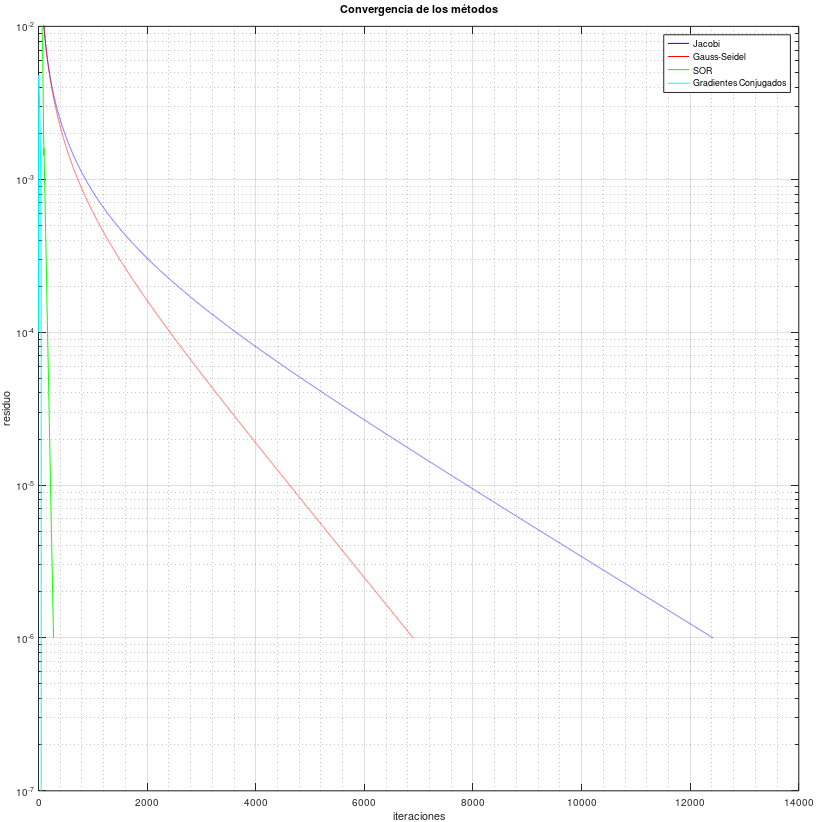
\includegraphics[scale=0.8]{ConvergenciaMetodos3}
\end{figure}

\newpage
Finalmente, se graficó la solución obtenida correspondiente a cada método, como una función $y=x(t)$
dónde t pertenece al intervalo [0,1].

\begin{figure}[h]
	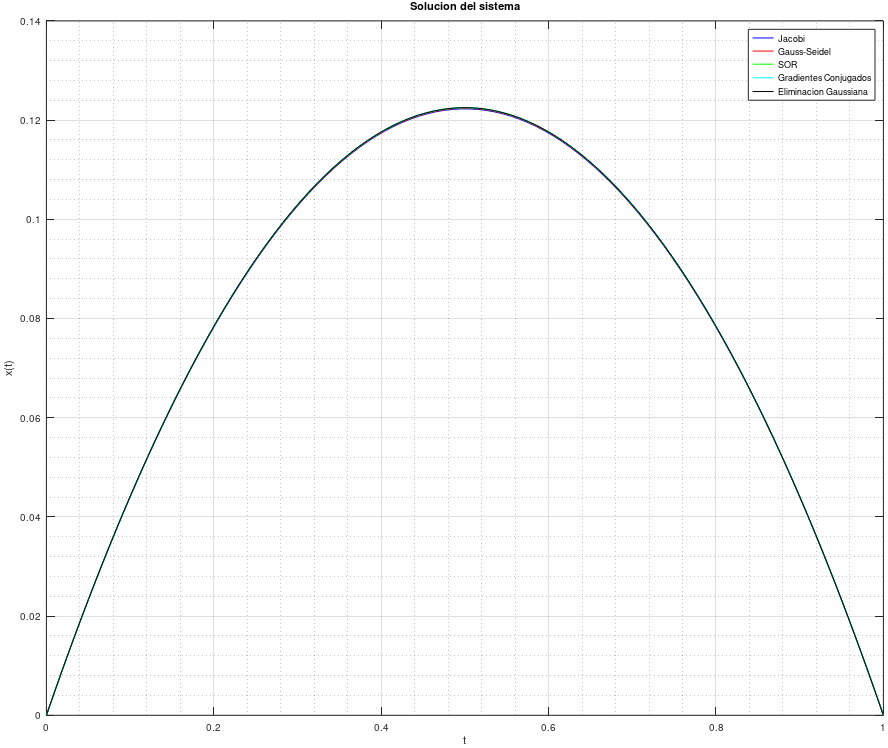
\includegraphics[scale=0.7]{SolucionDelSistema.png}
\end{figure}

\begin{figure}[!h]
	\centering
	\begin{minipage}{0.45\textwidth}
		\centering
		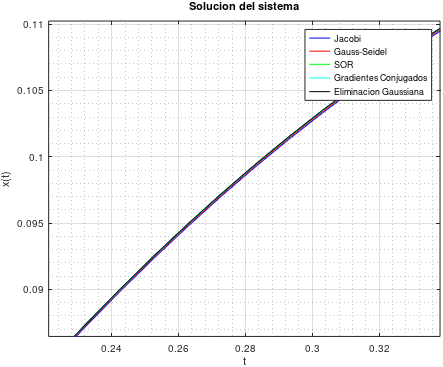
\includegraphics[width=0.9\textwidth]{SoluciondDelSistema1.png} % first figure itself
		\caption{Zoom 1}
	\end{minipage}\hfill
	\begin{minipage}{0.45\textwidth}
		\centering
		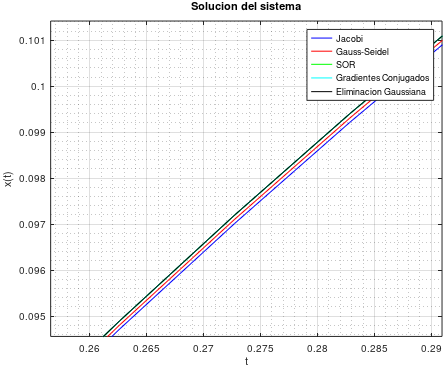
\includegraphics[width=0.9\textwidth]{SoluciondDelSistema2.png} % second figure itself
		\caption{Zoom 2}
	\end{minipage}
\end{figure}

\begin{figure}[h]
	\centering
	\begin{minipage}{0.45\textwidth}
		\centering
		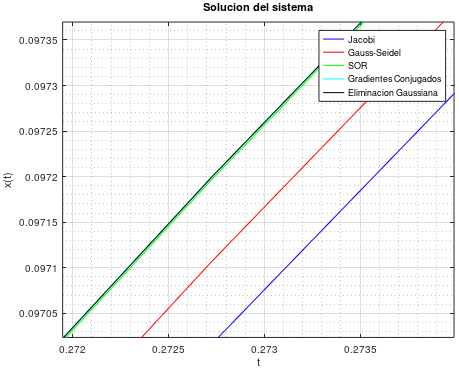
\includegraphics[width=0.9\textwidth]{SoluciondDelSistema3.png} % first figure itself
		\caption{Zoom 3}
	\end{minipage}\hfill
	\begin{minipage}{0.45\textwidth}
		\centering
		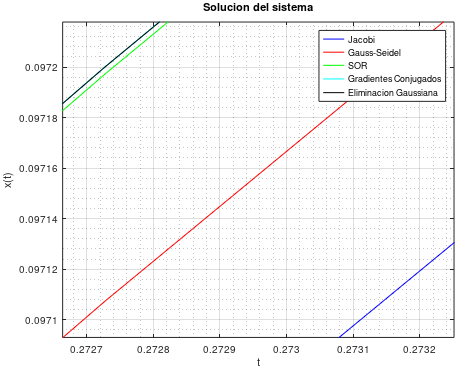
\includegraphics[width=0.9\textwidth]{SoluciondDelSistema4.png} % second figure itself
		\caption{Zoom 4}
	\end{minipage}
\end{figure}

\begin{figure}[!h]
	\centering
	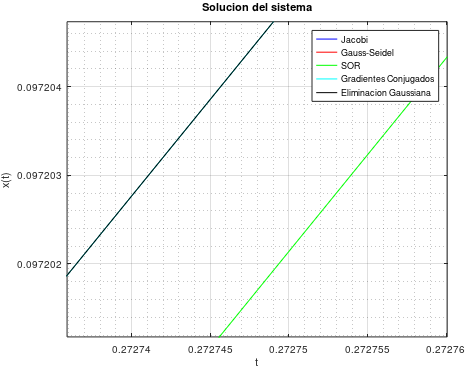
\includegraphics[scale=0.8]{SoluciondDelSistema5.png}
	\caption{Zoom 5}
\end{figure}
\newpage

Aunque a primera vista puede parecer que las soluciones correspondientes a cada método
son iguales, al realizar zoom sucesivos se puede observar como estas son diferentes.
Se visualiza como en los métodos iterativos la diferencia radica en el orden de la tolerancia
elegida y la solución más se aproxima a la real según la velocidad de convergencia del método, en tanto, las soluciónes correspondientes a Gradientes Conjugados y Eliminación Gaussiana
son indistinguibles, pues, con estos se obtuvo la solución exacta. Esto se debe a la naturaleza directa de los métodos,
pese a que gradientes conjugados puede ser considerado iterativo por su estructura de solución, también puede considerarse
como directo, dado la escasa cantidad de iteraciones que necesita para su convergencia.
\newpage
\begin{center}																		%%%
	\newcommand{\HRule}{\rule{\linewidth}{0.5mm}}									%%%\left

	\vspace*{1.0cm}								%%%
	%%%	
	\textsc{\huge \underline{ANEXO} \vspace{5px}}\\

\end{center}
\begin

\begin{lstlisting}[caption={gauss.m}]
function [x] = gauss(A,b)
	n=length(A(1,:));

	for k=1:n
		m = A(k+1:n,k)/A(k,k);
		b(k+1:n) = b(k+1:n) - m*b(k);
		A(k+1:n,k:n) = A(k+1:n,k:n) - m*A(k,k:n);
	endfor

	x=sust_atras(A,b);
endfunction
\end{lstlisting}

\begin{lstlisting}[caption={jacobi.m}]
function[x,it,r_h,t] = jacobi(A,b,x0,tol,maxit)
	%Calculo longitud del vector b
	tic();
	n =length(b);
	it=1;
	error =1;
	r_h = [];
	x = x0;
	while(it<maxit && error > tol)
	  %Aplico formula
	  for i=1:n
		x(i) = (b(i) - A(i,1:i-1)*x0(1:i-1) - A(i,i+1:n)*x0(i+1:n))/A(i,i);
	  endfor
	  %Calculo error 
	  error = norm(x-x0,inf)/norm(x,inf);
	  %Truco para guardar errores
	  r_h = [r_h ; error];
	  x0 = x;
	  ++it;
	endwhile
	t=toc()
endfunction
\end{lstlisting}

\begin{lstlisting}[caption={gauss\_seidel.m}]
function[x,it,r_h,t] = gauss_seidel(A,b,x0,tol,maxit)
	%Calculo longitud del vector b
	tic();
	n =length(b);
	it=1;
	error =1;
	r_h = [];
	x = x0;
	while(it<maxit && error > tol)
	  %Aplico formula
	  for i=1:n
		%El cambio con Jacobi es que aca hago uso del vector corriente 
		x(i) = (b(i) - A(i,1:i-1)*x(1:i-1) - A(i,i+1:n)*x0(i+1:n))/A(i,i);
	  endfor
	  %Calculo error 
	  error = norm(x-x0,inf)/norm(x,inf);
	  r_h = [r_h ; error];
	  x0 = x;
	  ++it;
	endwhile
	t = toc();
endfunction
\end{lstlisting}

\begin{lstlisting}[caption={SOR.m}]
function[x,it,r_h,t] = SOR(A,b,x0,tol,maxit,w)
	tic();
	%Calculo longitud del vector b
	n =length(b);
	it=1;
	error =1;
	r_h = [];
	x = x0;
	while(it<maxit && error > tol)
	  %Aplico formula
	  for i=1:n
		x(i) = (1-w)*x(i)+w*(b(i)-A(i,1:i-1)*x(1:i-1)-
		A(i,i+1:n)*x0(i+1:n))/A(i,i);
	  endfor
	  %Calculo error 
	  error = norm(x-x0,inf)/norm(x,inf);
	  %Truco para guardar errores
	  r_h = [r_h ; error];
	  x0 = x;
	  ++it;
	 endwhile
	 t = toc();
endfunction
\end{lstlisting}

\begin{lstlisting}[caption={GradienteConjugado.m}]
function [x, it, rh, t] = GradienteConjugado(A, b, x, maxit, tol)
  tic();
  residuo= b - A*x;
  v = residuo;
  c = residuo'*residuo;
  for it=1 : maxit
    if norm(v) < tol
      break;
    endif
    z = A*v;
    t = c/(v*z);
    x = x + t*v;
    residuo -= t*z;
    d = residuo'*residuo;
    rh(it) = norm(residuo,2);
    if rh(it) < tol
      break;
    endif
    v = residuo + d/(c*v)
    c = d;
  endfor
  t = toc();
 endfunction
\end{lstlisting}

\begin{lstlisting}[caption={TPentregable1.m}]
%Para el vector solucion x0,xN=0
N=100;
[A,b,x0]=crearMatriz(N);
tol=10^-6;
maxit=15000;
w = 1.5;

% a) y b)

%Jacobi
[xJacobi,itJacobi,r_hJacobi] = jacobi(A,b,x0,tol,maxit);
[TJacobi, cJacobi, tJacobi]=Tc_Jacobi(A,b,x0);
%Gauss-Seidel
[xGS,itGS,r_hGS] = gauss_seidel(A,b,x0,tol,maxit);
[TGS, cGS, tGS]=Tc_GaussSeidel(A,b);
%SOR
%Determinacion de parametro de relajacion para SOR
wsor = linspace(1.4,2,10);
vit=[];%Vector de iteraciones
for j=1:length(wsor)
  [xSor,itSor,r_hSor,tSor] = SOR(A,b,x0,tol,maxit,wsor(j));
  vit(j)=itSor;
 endfor
 dato = [wsor;vit]';%'
 [val pos] = min(dato(:,2));
 display("El parametro de relajacion optimo para SOR es ");
 w = wsor(pos)
 [TSor, cSor, tSor] = Tc_SOR(A, b, w);
 [xSorMin,itSorMin,r_hSorMin,tSorMin] = SOR(A,b,x0,tol,maxit,w);
%GradienteConjugado
[xGC, itGC, rhGC, tGC] = GradienteConjugado2(A, b, x0, maxit, tol);
%EliminacionGauss
[xGauss,itGauss] = gauss(A,b);

%Calculo de radios espectrales de las matrices de iteracion
display("Radio espectral matriz iteracion Jacobi");
radioJacobi = max(abs(eig(TJacobi)))
display("Radio espectral matriz iteracion Gauss-Seidel");
radioGS = max(abs(eig(TGS)))
display("Radio espectral matriz iteracion SOR");
radioSor = max(abs(eig(TSor)))  

%Muestra iteraciones
display("Iteraciones Jacobi");
itJacobi
display("Gauss-Seidel");
itGS
display("SOR");
itSorMin
display("Gradientes Conjugados");
itGC
display("Eliminacion Gauss");
itGauss

%Grafico de cada residuo
figure(1)
semilogy(r_hJacobi,'-b;Jacobi;')
ylim([10^(-7) 10^(-2)])
grid on 
grid minor
hold on
semilogy(r_hGS,'-r;Gauss-Seidel;')
semilogy(r_hSorMin,'-g;SOR;')
semilogy(rhGC,'kc;Gradientes Conjugados;')
title('Convergencia de los metodos')
xlabel('iteraciones')
ylabel('residuo')
hold off

%c)
%Grafico de las soluciones
d = linspace(0,1,100);

figure(2)
plot(d,xJacobi,'-b;Jacobi;')
grid on
grid minor
title('Solucion del sistema')
xlabel('t')
ylabel('x(t)')
hold on
plot(d,xGS,'-r;Gauss-Seidel;')
plot(d,xSorMin,'-g;SOR;')
plot(d,xGC,'-c;Gradientes Conjugados;')
plot(d,xGauss,'-k;Eliminacion Gaussiana;')
hold off

\end{lstlisting}

\end{document}

